
\subsection{PDRによる位置推定}

本ライブラリの基本的なPDR処理は,複数のクラスが協調して動作する設計となっている.
実装においてはコードの保守性と拡張性を重視し,Pythonの型ヒントやPandasライブラリを
効果的に活用している.特にPandasのデータフレーム構造を採用しており
大量のセンサデータに対する効率的な操作を実現している.また時系列データのリサンプリングや
欠損値の補間,データの結合などの操作が容易に行えるため,センサデータの前処理や
解析に要する実装の複雑さを大幅に削減できる.
図\ref{fig:pdr-class}に示すように,PDREstimatorを中心として,StepEstimator,
OrientationEstimator,TrajectoryCalculatorの3つの主要なクラスが連携して
位置推定を行う.
またセンサデータの管理はEnhancedSensorDataクラスが担当する.

\begin{figure}[H]
    \centering
    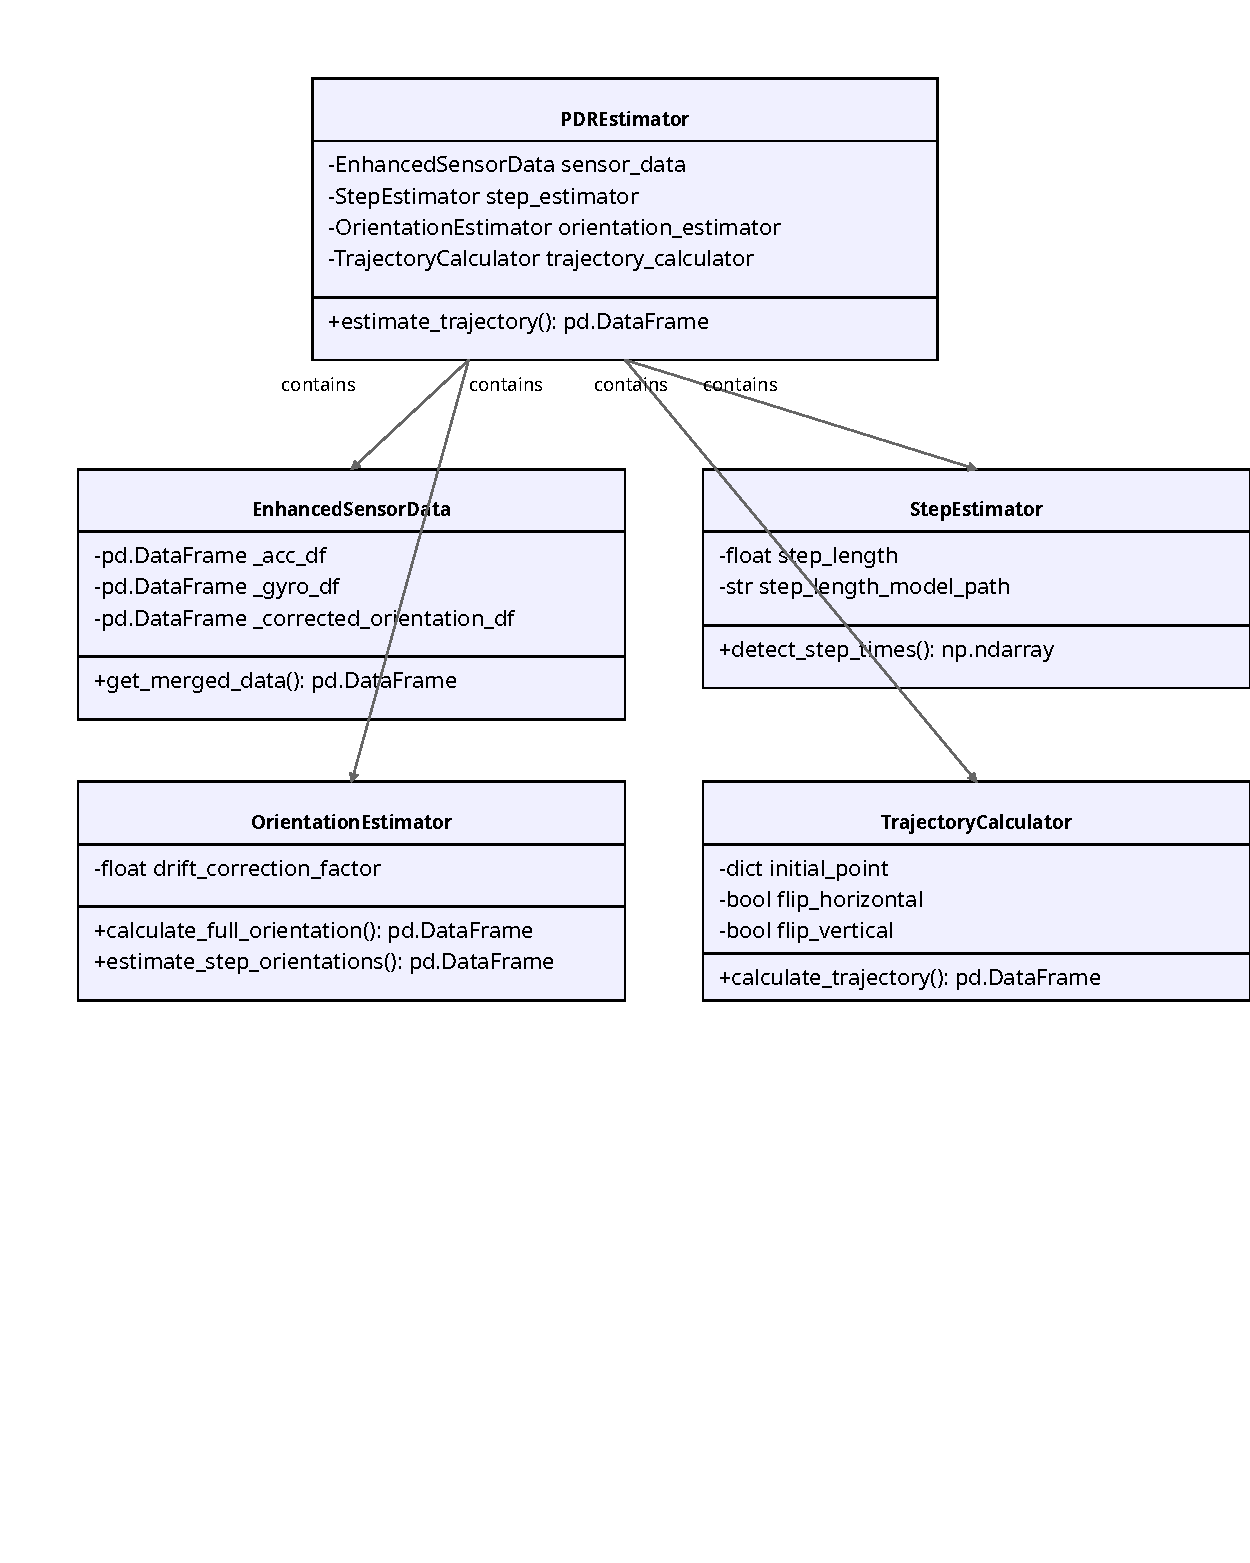
\includegraphics[width=\linewidth]{../image/pdr_figure.pdf}
    \caption{PDRの主要クラス構成}
    \label{fig:pdr-class}
\end{figure}
% TODO:2.こっちもbuilderパターンを採用してもよさそうな気がしてきた
% TODO:3.図の文字が小さくて読めない,図を大きくするといいかも

\subsubsection{システム構成}
% TODO:2. PDRのシステム構成かも?これだと全体のように見える

本ライブラリはクラスベースの設計を採用している.各クラスの責任範囲を
明確に分離しコードの理解性と保守性を向上させている.さらに拡張可能な
インターフェース設計を採用しており,各クラスは明確なインターフェースを通じて相互に
連携するため,個々の実装の詳細を隠蔽しながら機能拡張が可能である.
システムの中核となるPDREstimatorクラスは,歩行検出,方向推定,軌跡計算の
各処理を適切に連携させ最終的な位置推定を実行する統括的な役割を担う.
このクラスと連携するEnhancedSensorDataクラスは,加速度やジャイロセンサなどのセンサデータを
一元管理しデータの前処理や同期処理を行った上で,他のコンポーネントに適切な形式で
データを提供する.
歩行検出,歩幅推定を担うStepEstimatorクラスは加速度データから歩行ステップを検出,歩幅の推定機能を実装している.
またOrientationEstimatorクラスは角速度データから進行方向を推定し,
ドリフト補正などの基本的な補正処理も担当する.
これらの処理結果を統合するTrajectoryCalculatorクラスは,
検出された歩行ステップと推定された方向から実際の移動軌跡を計算する.
この計算結果は最終的な位置推定のための基礎データとして活用される.

\subsubsection{処理フロー}
PDRによる位置推定の処理フローを図\ref{fig:pdr-flow}に示す.
本ライブラリではセンサデータの
入力から最終的な軌跡の出力まで,以下の具体的な手順で処理を実行する.
まずEnhancedSensorDataクラスにおいて,加速度センサと角速度センサから取得した生データの
前処理が行われる.前処理ではデータの同期やノイズ除去などの基本的な処理に加え,
後続の処理で扱いやすい形式への変換が行われる.
具体的には加速度データと角速度データの
サンプリング周波数の違いを考慮し時系列データの補間処理を行い,両者のタイムスタンプを
一致させる.これにより後続の処理での時系列データの扱いが容易になる.

% TODO 3.図がおかしいので絶対修正する
\begin{figure}[H]
    \centering
    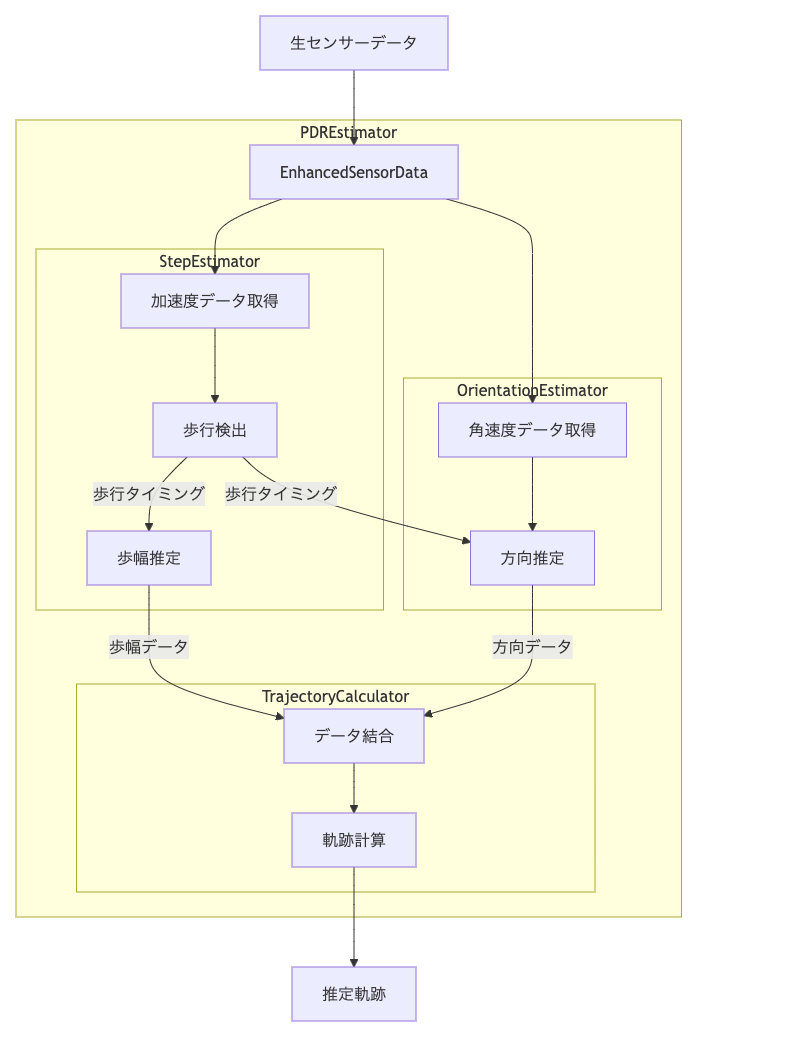
\includegraphics[width=\linewidth]{../image/pdr_flow2.png}
    \caption{PDRの処理フロー}
    \label{fig:pdr-flow}
\end{figure}


次にStepEstimatorクラスにおいて歩行ステップの検出と歩幅の推定を行う.
図\ref{fig:step_detect}に示すように歩行ステップの検出では3軸加速度の
ノルムを計算し,その値が閾値を超えた時点を歩行ステップとして検出する.
具体的にはまず加速度のノルムに対して平滑化処理を適用し,
ノイズの影響を軽減する.閾値は単純な固定値ではなく
システムは加速度信号の特性を逐次的に分析し,
平均値と標準偏差を用いて動的に閾値を調整する動的な閾値処理を採用している.
図\ref{fig:step_detect}の赤い破線で示されているように,
閾値は加速度の平均値に標準偏差の一定倍を加えた値として計算される.
この動的な閾値の採用により,歩行速度の変化や個人差による加速度パターンの
違いに柔軟に対応できる.また信号の品質が時間とともに変化する  % TODO:柔軟に対応はできてない.ある程度はぐらいの表現の方がよさそう.後品質は少し違和感
場合でも歩行検出が可能となる.
図中の赤い点が,この動的な閾値処理によって検出された歩行ステップを示している.
歩幅の推定ではあらかじめ学習済みのモデルを用いる方式と,固定値を用いる方式の
2つの手法を実装している.学習済みモデルを使用する場合は,各歩行ステップにおける
加速度のノルムと方向の変化量を特徴量として歩幅を予測する.一方学習済みモデルが
利用できない環境では,デフォルトの固定歩幅を使用する.
またこの固定値は外部のパラメータで変更可能である.

同時にOrientationEstimatorクラスでは角速度データを用いた方向推定を行う.
図\ref{fig:step_timing}に示すように角速度の積分により進行方向を算出する.
図中の青線は推定された進行方向の変化を,赤点は各歩行ステップでの方向を示している.
ただし積分処理には誤差の蓄積(ドリフト)の問題が存在する.
そのため本実装ではあらかじめドリフトの値が判明している場合,値を設定し線形ドリフト補正を適用できるようにしている.% TODO: できるようにしているは冗長かな
具体的には時間経過に比例する形でドリフト量を推定し,その影響を除去する処理を行う.

OrientationEstimatorクラスでは,まずジャイロセンサーから得られる角速度データを積分して全体の方向変化を計算する.
その後StepEstimatorから受け取った歩行タイミングに基づいて,
各歩行ステップでの方向を抽出する.これにより歩行ステップごとの進行方向が得られる.
図3.5に示すように青線は角速度の積分により得られた連続的な方向変化を表し,
赤点は各歩行ステップにおける方向を示している.

\begin{figure}[H]
	\centering
	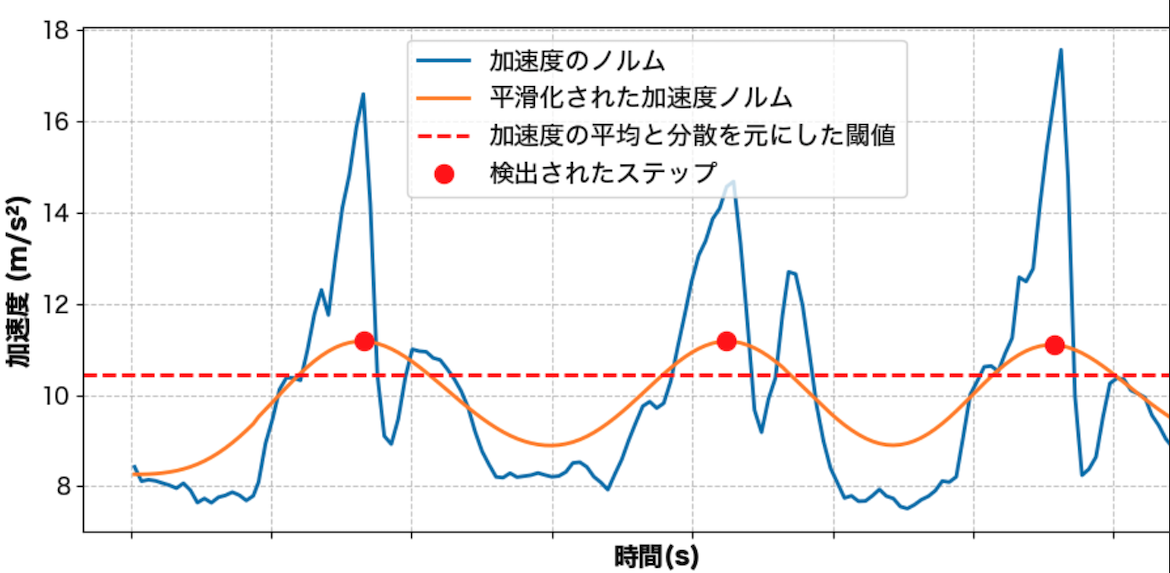
\includegraphics[width=\linewidth]{../image/step_detect.jpg}
	\caption{加速度を利用したステップ検出}    \label{fig:step_detect}
\end{figure}
% TODO: 2.下の図は時間に数値があるのにこちらにはない,統一した方がいい

\begin{figure}[H]
	\centering
	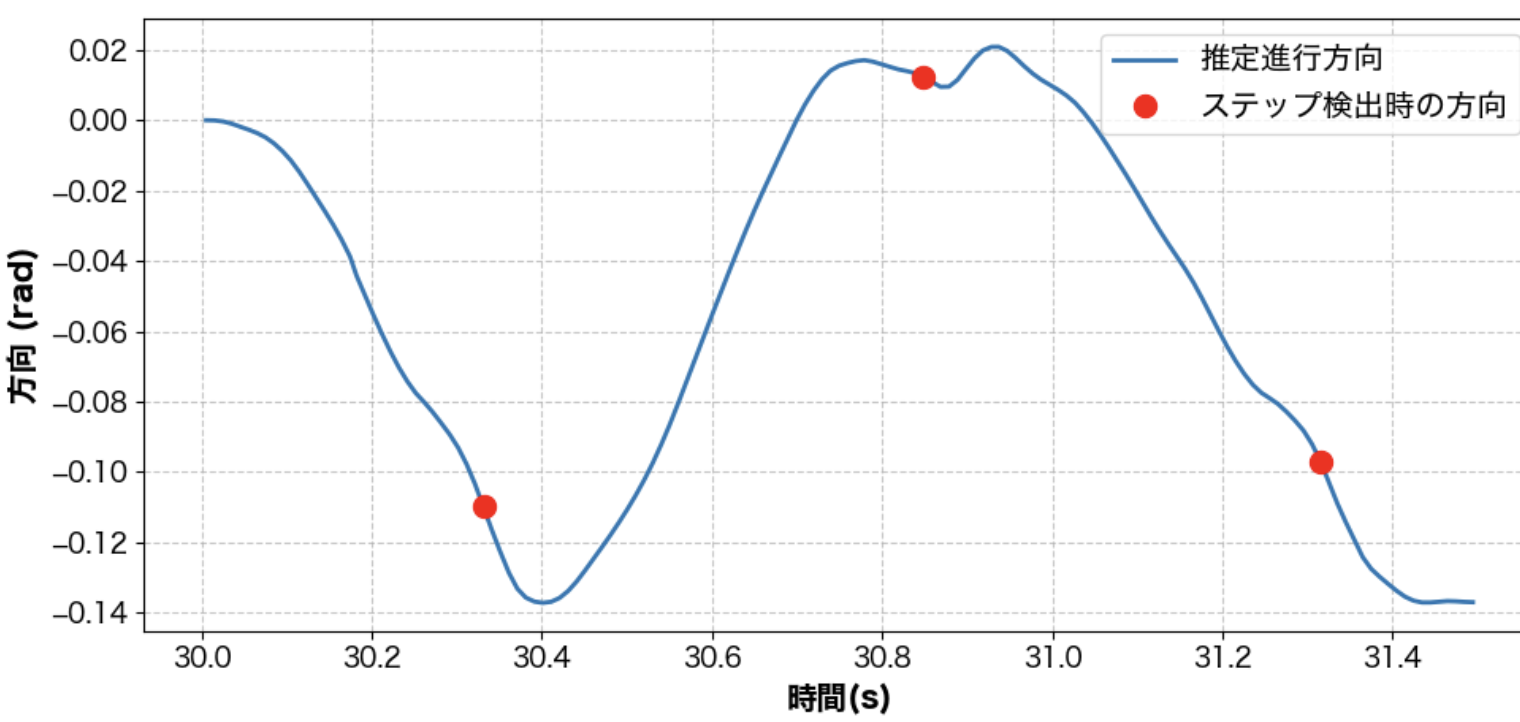
\includegraphics[width=\linewidth]{../image/step_timing_angle.jpg}
	\caption{推定進行方向の変化}    \label{fig:step_timing}
\end{figure}


% TODO:もう少し説明が欲しい
最後にTrajectoryCalculatorクラスにおいて検出された歩行ステップと推定された歩幅,
方向の情報を組み合わせて実際の移動軌跡を計算する.この過程では式\ref{eq:x_update}および式\ref{eq:y_update}に示す式を用いて座標を逐次的に更新する.
ここで$(x_n, y_n)$は$n$番目のステップでの位置,$L$は歩幅,$\theta_n$はその時点での
推定進行方向を表す.また初期位置が与えられている場合は,その値を$(x_0, y_0)$として
使用する.さらに座標系の定義に応じて必要な座標変換(x軸やy軸の反転など)も
この段階で適用される.


% TODO: 2.ここに中間報告で使用した計算が積み重なっていくのがわかる図があるといいかも

\begin{equation}
\label{eq:x_update}
x_{n+1} = x_n + L \cos(\theta_n)
\end{equation}
\begin{equation}
\label{eq:y_update}
y_{n+1} = y_n + L \sin(\theta_n)
\end{equation}


このように各クラスが明確な役割分担の下で連携し,PDRによる位置推定を
実現している.またこの設計により各処理段階での改良や機能追加が容易となっている.
例えばより高度な歩行検出アルゴリズムの導入や新たな方向推定手法の実装などを,
他のコンポーネントに影響を与えず可能である.


% TODO: 正解初期座標より既知の初期座標の方がいいかも
xDR Challenge 2023で与えられたトレーニングセンサーデータに対して処理を行った例を示す.
図\ref{fig:pdr}はPDREstimatorによる位置推定を行った結果である.
この図は2次元座標上に推定軌跡を表しており,軌跡の色は経過時間を表している.
紫色から赤色への変化が時間の経過を示している.
TrajectoryCalculatorに正解初期座標を与えた結果が図\ref{fig:pdr-move}である.
この図から分かるように,あらかじめ初期正解座標が判明している場合はPDRによる軌跡の初期位置を
適切に補正できる.比較のため,LiDARで取得した座標を基に出力された
軌跡を図\ref{fig:gt-trajectory}に示す.これを本論では正解軌跡として扱う.
図\ref{fig:pdr-move}と図\ref*{fig:gt-trajectory}を比較すると,初期位置を補正した
PDRによる軌跡であっても,正解軌跡と比べて大きく異なっているのが分かる.
これはPDR特有の問題として相対的な移動の累積による軌跡の歪みと,
実世界の座標系における正確な位置を特定する課題が存在するためである.
続く3.2.2節ではこれらの問題に対して軌跡補正クラスを用いたアプローチを示し,
PDRの軌跡を正解軌跡に近づけていく手法について詳しく説明する.


% TODO: この図1つにまとめてもいいかも,見づらい

\begin{figure}[H]
    \centering
    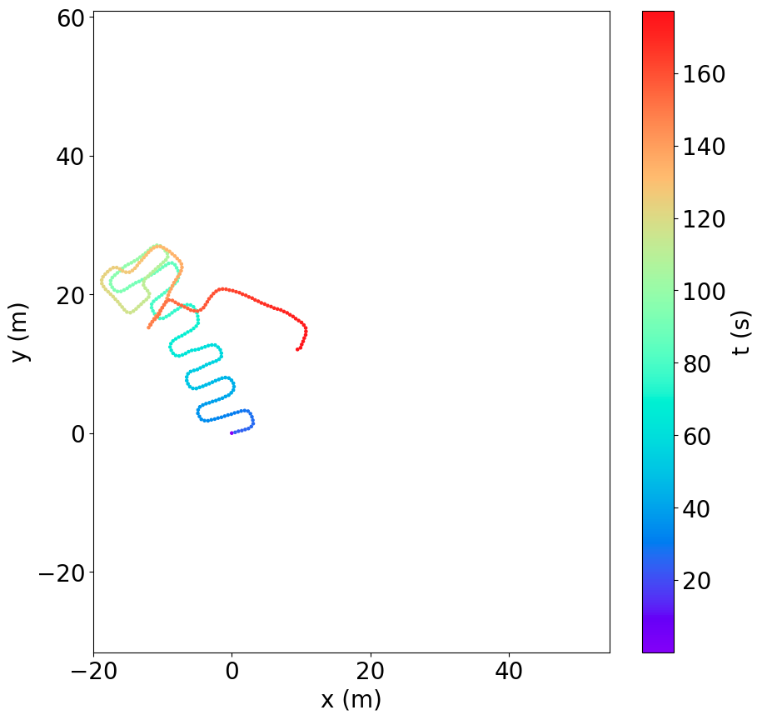
\includegraphics[width=\linewidth]{../image/pdr.jpg}
    \caption{PDREstimatorを用いた推定軌跡}    \label{fig:pdr}
\end{figure}

\begin{figure}[H]
    \centering
    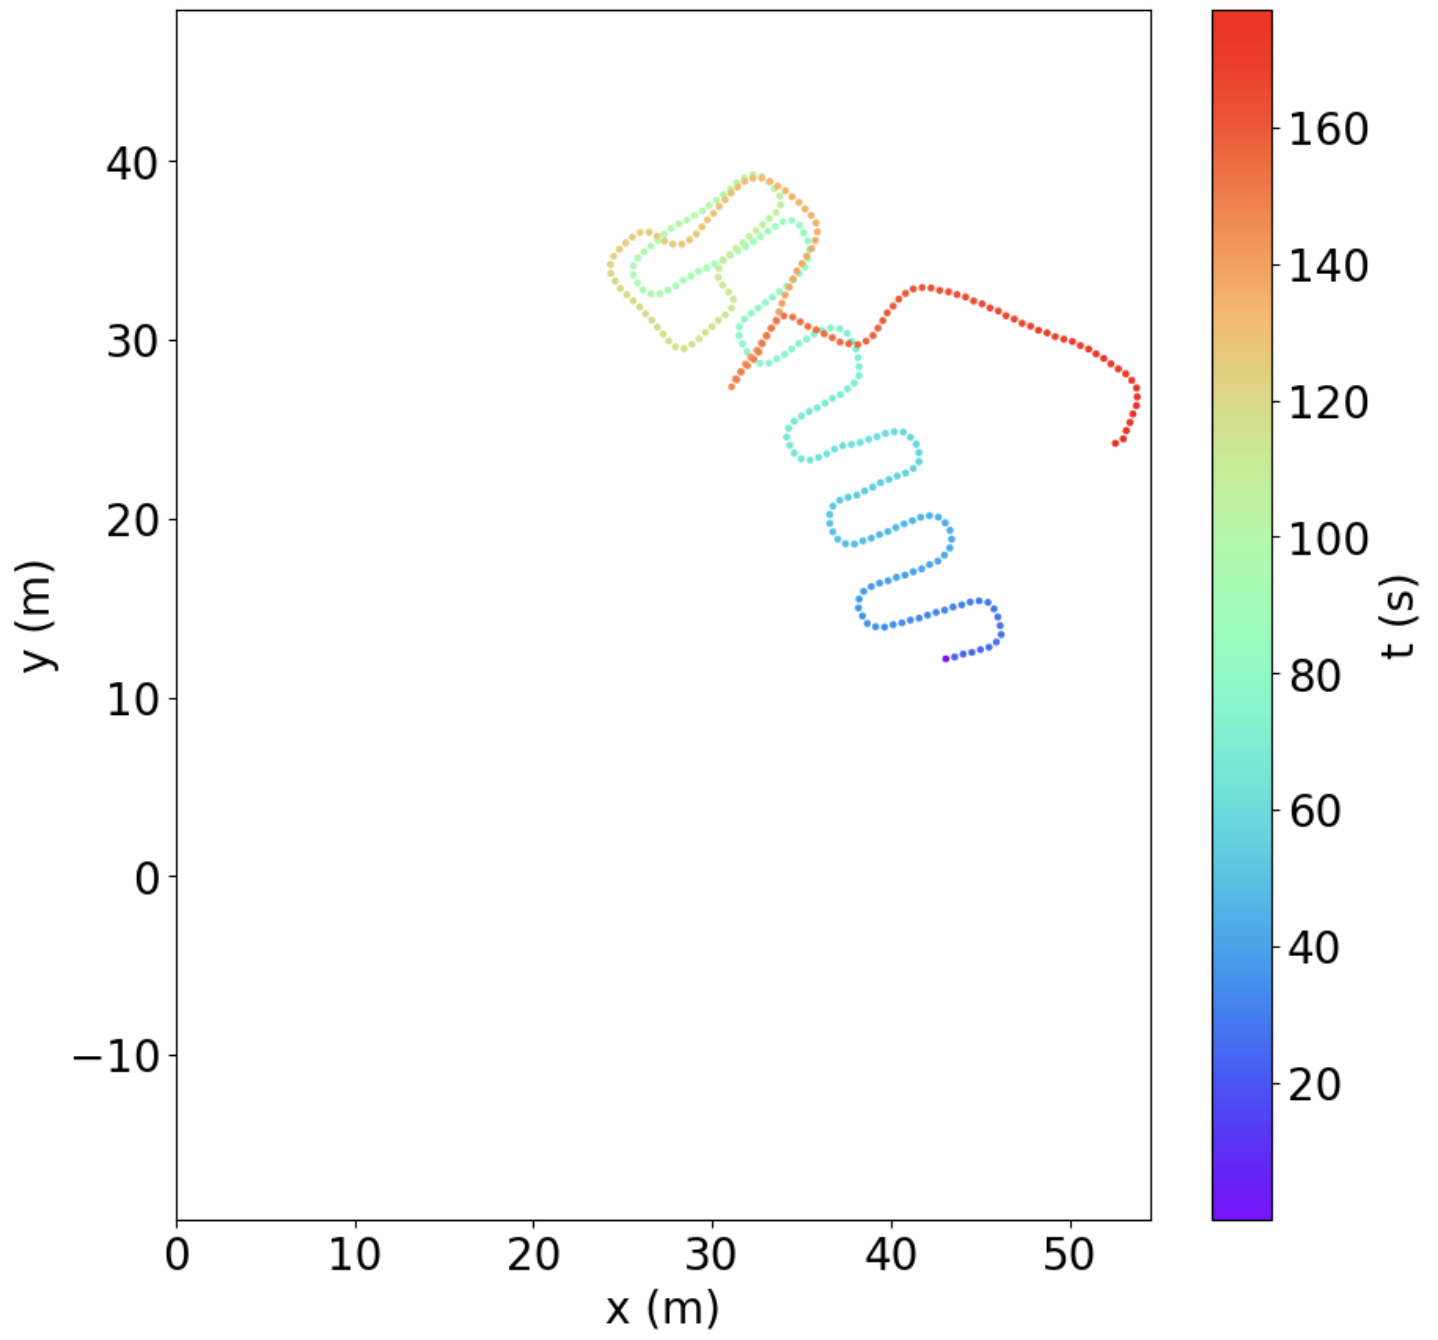
\includegraphics[width=\linewidth]{../image/pdr-move.jpg}
    \caption{正解初期座標が存在}    \label{fig:pdr-move}
\end{figure}


\begin{figure}[H]
    \centering
    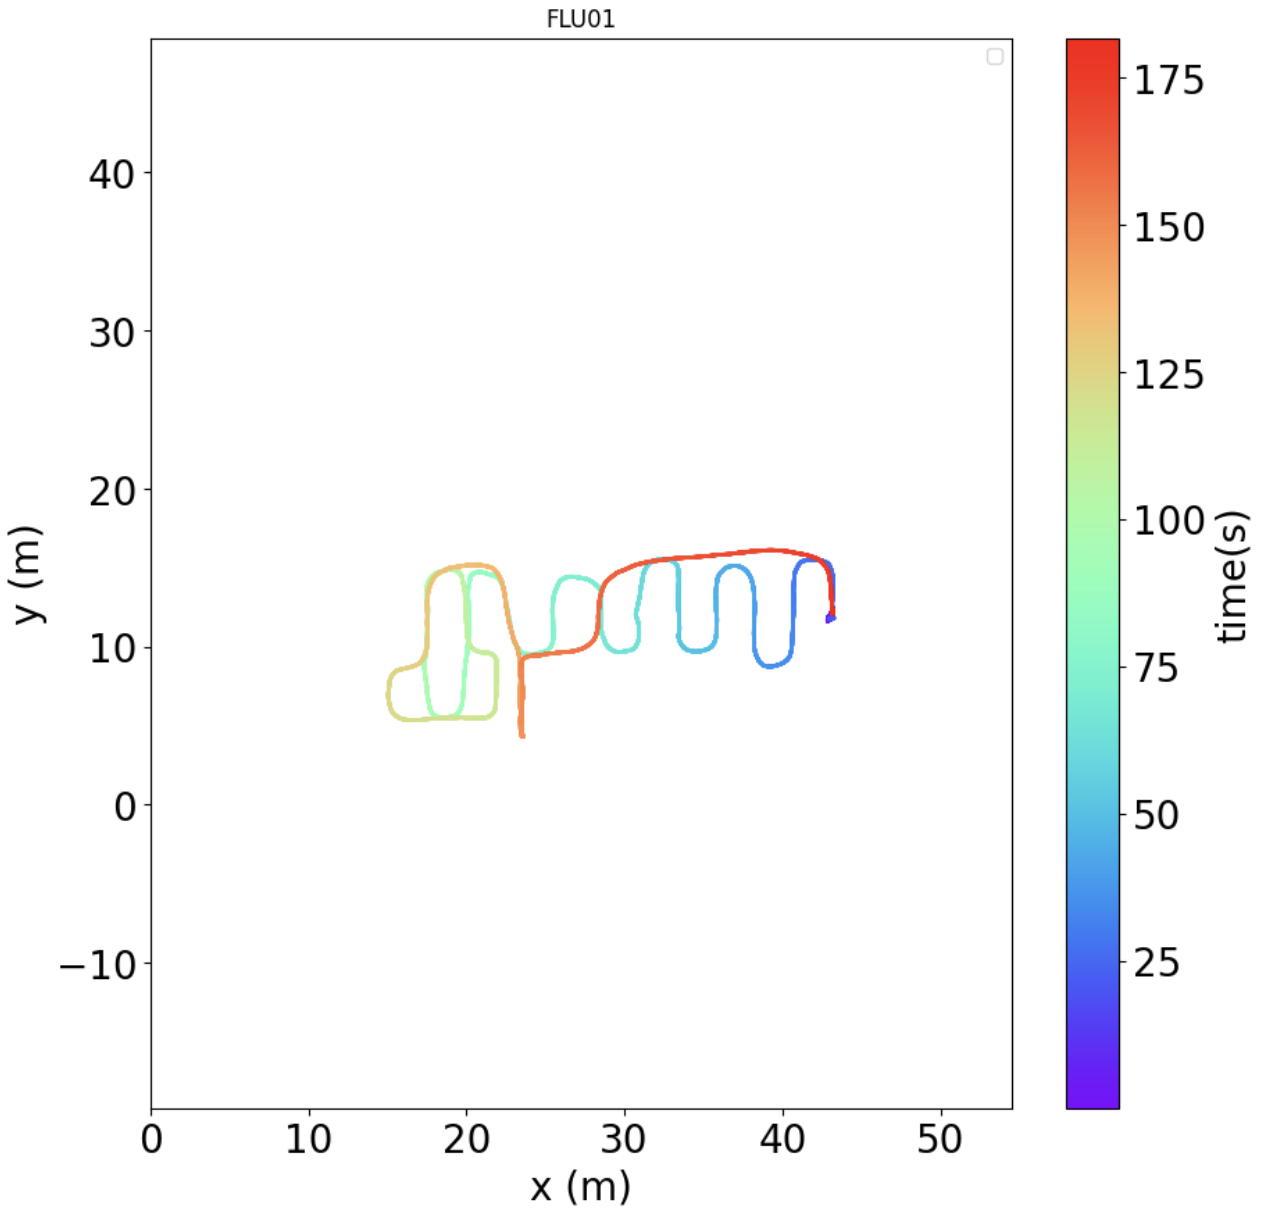
\includegraphics[width=\linewidth]{../image/gt2.jpg}
    \caption{正解軌跡}    \label{fig:gt-trajectory}
\end{figure}




